% This is samplepaper.tex, a sample chapter demonstrating the
% LLNCS macro package for Springer Computer Science proceedings;
% Version 2.20 of 2017/10/04
%
\documentclass[runningheads]{llncs}
%
\usepackage{graphicx}
\graphicspath{ {./img/} }

% Copyright 2017 Sergei Tikhomirov, MIT License
% https://github.com/s-tikhomirov/solidity-latex-highlighting/

\usepackage{listings, xcolor}

\definecolor{verylightgray}{rgb}{.97,.97,.97}

\lstdefinelanguage{Solidity}{
	keywords=[1]{anonymous, assembly, assert, balance, break, call, callcode, case, catch, class, constant, continue, constructor, contract, debugger, default, delegatecall, delete, do, else, emit, event, experimental, export, external, false, finally, for, function, gas, if, implements, import, in, indexed, instanceof, interface, internal, is, length, library, log0, log1, log2, log3, log4, memory, modifier, new, payable, pragma, private, protected, public, pure, push, require, return, returns, revert, selfdestruct, send, solidity, storage, struct, suicide, super, switch, then, this, throw, transfer, true, try, typeof, using, value, view, while, with, addmod, ecrecover, keccak256, mulmod, ripemd160, sha256, sha3}, % generic keywords including crypto operations
	keywordstyle=[1]\color{blue}\bfseries,
	keywords=[2]{address, bool, byte, bytes, bytes1, bytes2, bytes3, bytes4, bytes5, bytes6, bytes7, bytes8, bytes9, bytes10, bytes11, bytes12, bytes13, bytes14, bytes15, bytes16, bytes17, bytes18, bytes19, bytes20, bytes21, bytes22, bytes23, bytes24, bytes25, bytes26, bytes27, bytes28, bytes29, bytes30, bytes31, bytes32, enum, int, int8, int16, int24, int32, int40, int48, int56, int64, int72, int80, int88, int96, int104, int112, int120, int128, int136, int144, int152, int160, int168, int176, int184, int192, int200, int208, int216, int224, int232, int240, int248, int256, mapping, string, uint, uint8, uint16, uint24, uint32, uint40, uint48, uint56, uint64, uint72, uint80, uint88, uint96, uint104, uint112, uint120, uint128, uint136, uint144, uint152, uint160, uint168, uint176, uint184, uint192, uint200, uint208, uint216, uint224, uint232, uint240, uint248, uint256, var, void, ether, finney, szabo, wei, days, hours, minutes, seconds, weeks, years},	% types; money and time units
	keywordstyle=[2]\color{teal}\bfseries,
	keywords=[3]{block, blockhash, coinbase, difficulty, gaslimit, number, timestamp, msg, data, gas, sender, sig, value, now, tx, gasprice, origin},	% environment variables
	keywordstyle=[3]\color{violet}\bfseries,
	identifierstyle=\color{black},
	sensitive=false,
	comment=[l]{//},
	morecomment=[s]{/*}{*/},
	commentstyle=\color{gray}\ttfamily,
	stringstyle=\color{red}\ttfamily,
	morestring=[b]',
	morestring=[b]"
}

\lstset{
	language=Solidity,
	backgroundcolor=\color{verylightgray},
	extendedchars=true,
	basicstyle=\footnotesize\ttfamily,
	showstringspaces=false,
	showspaces=false,
	numbers=left,
	numberstyle=\footnotesize,
	numbersep=9pt,
	tabsize=2,
	breaklines=true,
	showtabs=false,
	captionpos=b
}


% copy the file from this repo
% Used for displaying a sample figure. If possible, figure files should
% be included in EPS format.
%
% If you use the hyperref package, please uncomment the following line
% to display URLs in blue roman font according to Springer's eBook style:
% \renewcommand\UrlFont{\color{blue}\rmfamily}

\begin{document}
%
\title{Ants-Review: A Protocol For Open Anonymous Peer-Reviews}
%
%\titlerunning{Abbreviated paper title}
% If the paper title is too long for the running head, you can set
% an abbreviated paper title here
%
\author{Bianca Trovò\inst{1,2}\orcidID{0000-0002-6776-2304}\thanks{Correspondent author: bianca.trovo@alumni.unitn.it} \and
Nazzareno Massari\inst{3,4}\orcidID{0000-0002-6638-2174}}
%
\authorrunning{B. Trovò et N. Massari}
% First names are abbreviated in the running head.
% If there are more than two authors, 'et al.' is used.
%
\institute{Sorbonne Université, Faculté des Sciences et Ingénierie, 75005 Paris, France \and
Neurospin research center, CEA/SAC/DSV/I2BM, 91191 Gif-sur-Yvette, France
\email{bianca.trovo@alumni.unitn.it}\\
\and
Alma Mater Politecnico di Torino, 10129 Turin, Italy\and
Independent Blockchain Engineer, London, UK \\
\email{nazzareno@nazzarenomassari.com}}
%
\maketitle              % typeset the header of the contribution
%
\begin{abstract}
Peer-review is a necessary and essential quality control step for scientific publications. However, the process, which is very costly in terms of time investment, not only is not remunerated but it’s also not recognized by the academic community as a relevant scientific output for a researcher. Therefore, scientific dissemination is affected. Here, to solve this issue, we propose a blockchain-based incentive protocol that rewards scientists also for their contributions to other scientists’ work and that builds up a reputational system. We designed a Protocol of smart contracts called Ants-Review that allows any author to issue a call for peer-reviewing their scientific publication. If requirements are met, peer-reviews will be accepted and payed by the Issuer. To promote ethical behaviour the system will implement an incentive mechanism on AntsReview.
\keywords{Blockchain  \and Open Science \and Privacy \and Peer-review \and Incentivization.}
\end{abstract}
%
%
\section{Introduction}
From its birth in 2008 as a distributed ledger for the peer-to-peer electronic cash system Bitcoin \cite{Bitcoin}, blockchain technologies (BCTs) have spread far beyond the sole cryptocurrency domain, in particular after the implementation of a general purpose smart contract functionality introduced by Ethereum \cite{Ethereum-Wood}.
Besides a growing number of applications ranging from business, healthcare, music industry, government, identity to cite but a few, blockchain technology has recently started to catalyse the attention of the scientific community as well \cite{Bitcoin-Nature-focus,vanRossum2017-DigSci} with the promising potential of being a 'game changer' in outdated and broken scientific practices and leading towards Open Science \cite{AES}. In particular, a 'blockchainified science'\cite{BlockchainforScience} could 'reduce waste'\cite{ReducingWaste-Lancet}, by disclosing each step the research cycle to 'scientific self-correction' way before the final publication step and therefore help fixing the current reproducibility crisis in science. Finally, scholars have pointed out how the intrinsic characteristics of blockchain technology (decentralization, for which there are no trusted third parties; cryptographic hashing and timestamping, that create a digital footprint able to keep a traceable chronological record of research objects; immutability or append-only, for which data cannot be altered or retrieved) set the basis for a open science infrastructure \cite{ReviewBlockchain2019} where decisional processes are transparent and therefore more democratically accessible to all the stakeholders (researchers, reviewers, funders, taxpayers).
A thorny issue in the academic system that can and should be tackled by blockchain concerns the status and accreditation of peer-review, the core process of scientific validation currently facing a crisis \cite{Gropp-PeerRevStress}. 
In this paper we propose a solution to the problem of reviewers recognition based on the principles of token economy and in line with the values of Open Science.
\newline The paper is structured as follows. Sections 2 presents research background and related works. Section 3 explains the proposed Ethereum-based protocol illustrating the system architecture and the current status of implementation. In Sect. 4 we discuss the implication of our work. Section 5 contains the conclusions. Appendixes present the smart contracts. 

\section{Background}
\subsection{Peer-review: present problems and mild solutions}
Peer review is still the only quality control mechanism devoted to evaluate scientific outcomes. The purpose of peer review is "improving the quality of the published paper, determining the originality of the manuscript, determining the importance of the findings, detecting fraud, and detecting plagiarism." \cite{Gropp-PeerRevStress}. However, the system is 'flawed' and outdated \cite{Smith2006} and presents multifaceted issues, here reviewed.
\paragraph{A slow multi-stage process.} The main issues affecting the effectiveness of peer-review is the delay between paper submission and journal acceptance for publication. The traditional peer-review process is completely controlled by the editor(s). The author(s) submit manuscript to the journal where an editorial team assesses if the paper meets meets the scopes of the journal and novelty criteria. If the editorial decision is to send the manuscript for review, the handling editor personally selects potential reviewers. The reviewers identity is usually only know to the editor but is hidden to the authors or the other reviewers themselves (single-blind review). Reviewers independently conduct their reviews by exposing in their reports strengths and weaknesses of the manuscript and sometimes substantially improving the draft. If the decision is a major or minor revision, authors are invited to re-submit a corrected or improved version of the manuscript with a letter to the reviewers. The same reviewers might be contacted again and if they want they can follow up the peer-review process. This process can take multiple rounds and is a huge time investment both for authors and reviewers. An analysis of all papers published in PubMed for a time period of 30 years claims that the median review time is around 100 days\cite{Kendall-peerrev}.
\paragraph{Social and cognitive biases.} Given the fact that anonymity is usually asymmetrically applied only for reviewers, many power related dynamics can influence the reviewers decision, such as gender or cultural discrimination, social prestige of the institution. To solve this problem some journals have implemented double-blind review process (identity of both authors and reviewers are masked) which seems to reduce the bias towards minorities.
\paragraph{Fraud and misconduct.} Due to the 'publish or perish culture' pressures, unethical behaviour from reviewers has been occasionally reported, from abusive behaviour towards authors \cite{Smith2006,tragedy-reviewers} to identity fraud. Some studies have reported an improvement in the transparency and 'civility; of the review process when open reports are released (open peer review). 
\paragraph{Peer reviews need to be...reviewed.} There is high variability in the reliability and depth of reviews and a recurrent question is: "Who watches the watchers?". 
\paragraph{Need for more reviewers.} There is a disproportion between the progressive increase in journals and the number of experienced reviewers assigned which demands an expansion of the reviewer's pool including early career scientists. \cite{tragedy-reviewers}.
\paragraph{Lack of recognition.} Peer-reviewing is an invisible activity purely conducted on voluntary basis, neither paid by the journals or officially credited via standard scientific metrics (such as the ones that establish the 'impact factor' of an author). Thus, it does not lead to advancements in career or help securing grants. Researchers are motivated in doing peer-review for a sense of belonging and a desire to 'give back' to the community. A major consequence of not promoting incentives for the quality (and quantity) of peer-reviews is to either slow down publication of potentially good research which awaits for validation or let bad science being published through sloppy and uncritical reviews.
Some mild attempts to credit peer review has been handled without much success by journals via attribution of virtual 'badges', certificates of performance, citation in annual editorials. It's worth mentioning: Publons\cite{Publons}a service integrated with ORCID (researcher identifier) that provides peer-review metric; Peerage of Science\cite{Peerage}, a journal-independent free service for scientific peer review and publishing that provides also a peer-review of the reviews.

\section{System concept}
In this paper we propose Ants-Review, a new incentivisation mechanism built on a distributed platform that issues open peer-reviews to validate scientific papers while preserving the anonymity of its contributors. We imagine a final paper originating from the peer-review process as a complex system that emerges from the interactions between the authors and the reviewers, a whole that is more than the sum of its parts. Therefore, the name evokes an ant colony as a self-organising organism in which all micro-contributions of the individuals emerge into complex behaviour.
A previous version of this paper can be found here \cite{AntsReview}.Its design and implementation are exposed in the following section.
Here we expose the main features of AntsReview:
\begin{itemize}
\item \emph{accountability}: both for recognition and for security against fraud and abuse etc we need to be able to track back the identities of the contributors to a peer-review to make sure there are no conflict of interest. This means the platform acts like a version control system where commit are permanent and hashed; 
\item \emph{transparency of the records}: all reviews should be open access to the community to prevent waste of knowledge and disrupt the secretive system of black boxes of peer reviews in journals that centralize all the reports 
\item \emph{incentivisation}: via symbolic and material recognition of the performed work. reputation and bounties
\item \emph{inclusiveness via gamification}: all the community is involved in the process - no selection process feeling of belonging -- quadratic voting and share of the stake
\end{itemize}
crowdfunding schemes leveraged by blockchain technology
In the following sections we describe the architecture of the system and its building blocks
AntsReview [Fig.\ref{fig:contracts}] is a distributed peer-review system which synthesizes successful ideas from previous systems including The Bounty Network \cite{Bounty}, ERC-20 \cite{ERC20}, AZTEC Protocol \cite{AZTEC}, IPFS \cite{IPFS}, Proof of Existence \cite{TimeStamp-Haber}, ...

\subsection{Design}

There are two possible scenarios depending if we save the role of the editor and we integrate an existing journal or if AntsReview becomes a platform completely decoupled from journals.

\subsubsection{AnstReview process: scenario 1 (journal-dependent)}

\begin{enumerate}
    \item The author submits a manuscript to the journal.
    \item If the papers passes stage 2-3 of editorial decision (appropriateness of style and coherence with the journal's scope)
    \item the editor issues a bounty (\emph{bounty issuance}) for the paper review. Fulfillment rules are set in a smart-contract.
    \item (footnote?) the bounty prize could correspond to part of the article submission fees and article publication fees requested to the authors by the journal.
    \item Reviews fulfilling the smart-contract requirements are validated by the journal editors.
    \item When the reviews are accepted (\emph{bounty fulfillment}), reviewers awarded a token called \emph{ANT}.
    \item Not all reviews will have the same quality and depth. However, each of them might bring up one or more relevant contribution for the sake of improving the manuscript. In order to redistribute the bounty in a fair manner across reviewers, reviews will be voted by Anters (members of the community) via Quadratic Voting to rank the most prolific peer-reviewers.

\end{enumerate}

\subsubsection{AnstReview process: scenario 2 (community-driven)}:

\begin{enumerate}
    \item The author submits a manuscript to the pre-print service or to an hypothetical AntsReview platform).
    \item The paper is accepted by the community for revision in its whatever format.
    \item The author issues a bounty (\emph{bounty issuance}) for the paper review. Fulfillment rules are set in a smart-contract.
    \item (footnote?) the bounty prize could come by a community stake that participates in the peer-review process either as a reviewer or as a reviewer checker.
    \item Reviews fulfilling the smart-contract requirements are validated by the AntsReview community/contributors.
    \item When the reviews are accepted (\emph{bounty fulfillment}), reviewers awarded a token called \emph{ANT}.
    \item Not all reviews will have the same quality and depth. However, each of them might bring up one or more relevant contribution for the sake of improving the manuscript. In order to redistribute the bounty in a fair manner across reviewers, reviews will be voted by the community via Quadratic Voting.
    \item In order to incentive 'fair play' also the review checkers who vote for the best quality reviews will share the final prize from the bounty. Since it's in their own interest to 'bet' on a good review, this gamed system will discourage internal dynamics prompt to favour specific members of the community beyond real personal merit. It will also fuel ethical behaviour.

 \end{enumerate}

\subsection{Implementation}

\begin{figure}
\centering
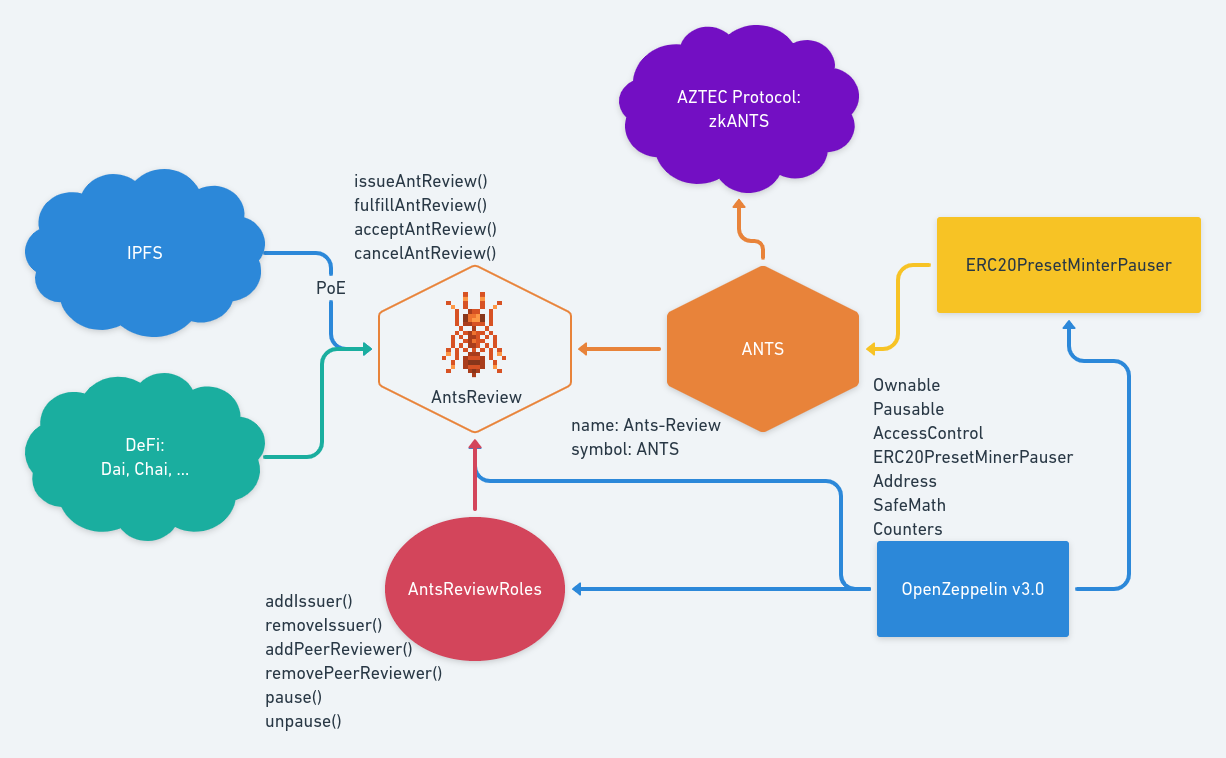
\includegraphics[scale=0.28]{AntsReview}
\caption{AntsReview Smart Contracts}
\label{fig:contracts}
\end{figure}
In this section we provide an overview of how we implemented the system by focusing on its components.

The AntsReview Protocol is divided into different modules responsible for the following functionalities as shown in the flow-chart [Fig. \ref{fig:contracts}]:

\begin{itemize}
\item AntsReview - manage access management and the basic system.
\item Tokenomics - manage system incentivization mechanism integrating ideas from DeFi and Quadratic Funding.
\item Privacy - maintains the anonymity of the system via AZTEC Protocol.
\end{itemize}

\subsubsection{AntsReview}

AntsReview \cite{Ant} is the core of the smart contracts deployed on Ethereum Rinkeby's Testnet \cite{Rinkeby}
\newline It implements a Bounty-like system where an issuer (author) is asked a series of actions, to ensure transparency and robustness, regarding the AntReview that he's creating:
\begin{itemize}
  \item to upload the file containing the requirements of the peer-review and the paper into IPFS\cite{IPFS}.
  \item to specify a deadline in the form of a unix timestamp after which the fulfillment will no longer be accepted.
  \item to send the amount of ether for the reward.
\end{itemize}

AntsReviewRoles, to ensure integrity of the system, implements an access management, leveraging on AccessControl.sol by OpenZeppelin Library \cite{OZ}, through the creation of the Roles Issuer and Peer-Reviewer.
\newline It also integrates a circuit breaker design pattern via Pausable.sol by OpenZeppelin to allow the Pauser Role, that by default is the Owner of the Smart Contracts, to pause (or unpause) the functions in case of emergency.
\newline In this way, only the Issuer (author) can create a new AntReview.
\newline Once created, an AntReview is available to be fulfilled by Peer-Reviewers, uploading the peer-review on IPFS before the deadline.
\newline The AntReview after being validated is then accepted by the Issuer and paid equally between Peer-Reviewers.
\newline Also, the Issuer can cancel the AntReview at any time and withdraw the amount of ether staked.
\newline One of the key aspects of the protocol is the concept of Proof of Existence, introduced by Stuart Haber \& W. Scott Stornetta with the paper "How to time-stamp a digital document"\cite{TimeStamp-Haber}
\newline As the pioneers of blockchain an cited by Bitcoin whitepaper, they were in a mission to solve the problem of immutability of digital records that became reality with the Blockchain and Bitcoin \cite{Bitcoin} as its first application.
\newline In Ethereum \cite{Ethereum} the concept of immutability is achieved via the blockchain and proof of work consesus algorithm by a chain of timestamped block hashes that are secured by miners competing computations.
\newline AntsReview is evaluating the advantages of storing the hashes of the peer-reviews into a Merkle Tree \cite{BayerHaber1992} to achieve immutability and efficiency in verifying the data with a complexity of O(logn) for searching through the tree.
\newline A Merkle tree is a particular type of binary tree, formed by a set of nodes with a large set of leaf nodes at the bottom of the tree containing representing the hash of the original data, a set of intermediate nodes where each node is the sum of the two children hashes, ending with a single root hash.
\newline In order to verify if a specific hash is included into a Merkle Tree, leveraging on MerkleProof.sol by OpenZeppelin Library, we need to provide a proof, generated from the leaf of interest, that represent the ramification derived from the leaf, the root hash and finally the leaf we want to verify.
\newline The paper and peer-review documents will be included into a Merkle Tree by hashing the data using keccak256, a cryptographic hashing algorithm available in Solidity \cite{Solidity}, an object-oriented programming language for writing smart contracts that run on the Ethereum Virtual Machine (EVM).

\subsubsection{Tokenomics}

AntsReview has few tokens, each of which plays an integral role in the functioning and anonymity of the decentralized protocol.
\newline Ant, is the primary protocol token and can be staked into an AntReview if you wish to provide the protocol with an additional security promise.
\newline Ant (as shown below) is implemented by inheriting ERC20PresetMinterPauser.sol from OpenZeppelin Library with name: \emph{Ant} ans symbol: \emph{ANT}.
\newline An AntReview, issued by an author will be seen as a poll where Anters (members of the AntsReview Community) can stake ether or tokens from DeFi services including Dai \cite{Dai}, Chai \cite{Chai}, ... with the possibility to accrue interest for the duration of an AntReview (1 year on average), via MakerDAO DSR (Dai Saving Rate) \cite{DSR} or Compound \cite{Compound} to cite a few.
\newline An AntsReview DAO will be formed in the future to allow Ant stakers the ability to participates in a Decentralized Autonomous Organization which will be used to govern important aspects of the decentralized protocol, from smart contracts upgrades to more minor changes in settings across the protocol.
\newline Hive. When an Anter deposits into an AntReview, they will instantly receive the Hive token which represents their deposit and the accrued interest it gains over time in the AntReview.
\newline This token doesn't need to be locked in the network and it can be traded, sold, or held as the Anter desires.
\newline Hive will be implemented using a similar approach to Ant and Chai, a token that accrues interest from MakerDAO's DSR or Compound, with name: \emph{Hive} and symbol: \emph{HIVE}
\newline Ideally, but is still under investigation, after the deadline of the AntReview is reached, the Hive token will be burned for Ant and wrapped into zkAnt to promote anonymity and sent equally to the peer-reviewers that fulfilled the AntReview.
\newline zkAnt, is an Ant token wrapped into AZTEC Protocol \cite{AZTEC} ZK-SNARKs, that will be extended to PLONK \cite{PLONK} Proof to collapse the gas costs of private transactions on mainnet.
\newline zkAnt will be implemented via AZTEC 2.0 (still in development) that will allow to securely wrap the Ant Token into zkAnt, allowing private transactions on mainnet and preserving the anonymity of Peer Reviewers.
\newline Finally, another concept under investigation is Quadratic Funding \cite{LiberalRadicalism}, used by Gitcoin \cite{Gitcoin} to match donations for Grants. This will allow to incentives prolific Peer-Reviewers and improve the stability of the system together with ideally a reward system to rank best Peer-Reviewers.


\begin{lstlisting}[language=Solidity]
/// SPDX-License-Identifier: GPL-3.0
pragma solidity 0.6.8;

///@title AntsReview
///@author Nazzareno Massari
///@notice Ant ERC20 Token
///@dev All function calls are currently implemented without side effecs through TDD approach
///@dev OpenZeppelin library is used for secure contract development

import "@openzeppelin/contracts/presets/ERC20PresetMinterPauser.sol";


contract Ant is ERC20PresetMinterPauser {

  constructor()
  ERC20PresetMinterPauser("Ant", "ANT")
  public {

  }

}
\end{lstlisting}


\subsubsection{Privacy}

The Anonymity of an agent in the system is achieved in two ways:

\begin{itemize}
  \item PseudoAnonimity granted by an Ethereum's Externally Owned Accounts (EOA) address that can pseudo-obscure the identity of the agent.
  \item Private Transactions allowed by AZTEC Protocol security layer via zkAnt. Future developments will allow to leverage on PLONK Proofs to reduce gas costs and improve scalability.
\end{itemize}

 Externally Owned Accounts (EOA) in Ethereum are controlled by private keys, are 20 bytes long and have no code. An user can send messages from an externally owned account by creating and signing a transaction.
\newline The limitation of such solution regarding the Privacy of the Protocol is due to the fact that blockchain and transactions are public so anyone can see the details of a transaction, browsing a block explorer like Etherscan, and also they're subjected to data mining to extract value and identify users in the blockchain.
\newline To avoid that, AntsReview will implement zkAnt, an Ant token wrapped into AZTEC Protocol, where leveraging on zkSNARKS, and PLONK in the future, will allow private transactions in the system to maintain the privacy and anonimity of Peer-Reviewers.
\newline The AZTEC Protocol was conceived to enable privacy on public blockchains. It uses a series of zero-knowledge proofs (ZK-SNARKs) and homomorphic encryption to validate encrypted transactions.
\newline ZK-SNARKs (Zero-Knowledge Succinct Non-Interactive Argument of Knowledge) \cite{ZKSNARKs} refers to a proof construction where one can prove possession of certain information, like a secret key, without revealing that information, and without any interaction between prover and verifier.
\newline Zero-Knowledge \cite{ZeroKnoledge} proof is a mathematical cryptographic method that through values permutations allow one party (the prover) to prove to another (the verifier) the validity of a statement, without revealing the statement itself.
\newline Future developments will investigate viable solutions, for scaling the system, like ZK-Rollups by AZTEC Protocol, one of the options being developed for a type of layer 2 construction that runs on top of Ethereum to improve scalability. This will enable to run smart contracts at scale with quasi-instant transactions while still being secured by Ethereum.

\section{Discussions}
\subsection{A new community-driven standard?}
- a change is already happening: specially new born publishers are opening up review process (BioMed Central, ELife, Frontiers, PeerJ, F1000 Research) -- from 2020 also Nature declared that will do the same.

- new business model? at some point pre-print platforms (dissemination) might want to integrate peer-review (validation) into their platforms - dissociation of initial scientific dissemination and scientific validation will force publishing industry to adapt: how will they justify their added value? as Tennant points out: branding archiving

- peer reviews requires a standard: building smart-contracts for peer-reviews might set a first step in this direction

- community-organized peer reviews: peer reviews will be more and more out of the hands of publishers, researchers will be the ones seeking the papers to review (like in Rubriq).

future of quality control and moderation: open participation model, community-driven | certification and reputation: expansion of reviewer pool with fewer barriers to enter and more inclusion of young scientists, reputation build within community and not journals

- portable peer review not only within a consortium of journals

-value of peer review as 'academic capital' recognized by research funders and hiring committees

-a bit off topic but: automated peer review (services such as StatReviewers) might fasten the formal aspects of the job allowing reviewers to focus on the content.

\subsubsection{Perspectives for a Decentralized Autonomous Organization (DAO)}

\section{Conclusion}
In this paper we addressed a crucial problem within scholarly academic communication: the peer-review process. We showed how blockchain technology could provide an efficient and viable solution to open up possible directions for a paradigm shift in scientific communication. We proposed an incentive mechanism that could solve the problems of lack of acknowledgment and trust during peer-reviews. We exposed the architecture of our project for which we adopted cutting-edge tools from the open source blockchain ecosystem.

\subsubsection{Supplementary material}
Source Code, DOI: 10.5281/ZENODO.3829162
\newline Demo (PoC), DOI: 10.5281/ZENODO.3829183

\subsubsection{CRediT Authorship Contribution Statement}
 Bianca Trovò: Conceptualization, Investigation, Writing - original draft, Writing - review \& editing. Nazzareno Massari: Project administration, Methodology, Validation, Software development, Visualization, Writing \& editing. Both authors equally contributed and supervised the project.

\subsubsection{Declaration of Competing Interest}
The authors declare no competing interests.

\subsubsection{Acknowledgements} We would like to thank Matteo A. Tambussi and Keno Budde for useful comments.


% ---- Bibliography ----
%
% BibTeX users should specify bibliography style 'splncs04'.
% References will then be sorted and formatted in the correct style.
%
\bibliographystyle{splncs04}
\bibliography{ref1-intro.bib, ref2-peerreview.bib, ref2-relatedwork.bib, ref3-system.bib}

\end{document}
